\documentclass[10pt]{article}
\usepackage[utf8]{inputenc}
\usepackage[T1]{fontenc}
\usepackage{amsmath}
\usepackage{amsfonts}
\usepackage{amssymb}
\usepackage[version=4]{mhchem}
\usepackage{stmaryrd}
\usepackage{graphicx}
\usepackage[export]{adjustbox}
\graphicspath{ {./images/} }

\begin{document}

    A quasar is an extremely luminous active galaxy powered by a supermassive black hole that emits relativistic jets. The figure shows a series of panels of radio images of a quasar (with redshift $z=0.53$, and luminosity distance $D_{\mathrm{L}}=1.00 \times 10^{10} \mathrm{ly}$ ) at different times. The "core" aligns with the vertical white line, while a jet, consisting of a "blob" (marked white +), moves away from it over time. Each panel shows the observation time (starting with $T_{0}$ for the first image), and the angular scale is indicated at the top and bottom of the figure.\\
    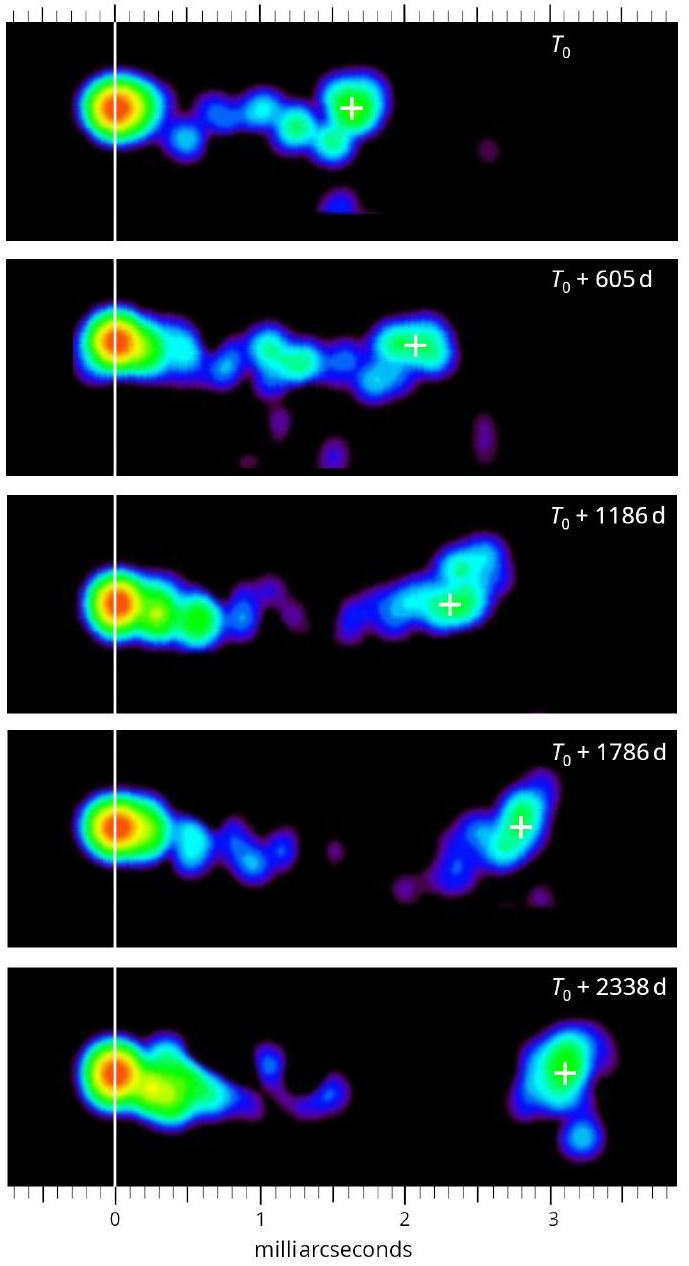
\includegraphics[max width=\textwidth, center]{2025_08_23_e94579452776a99c4850g-03}\\
    (T05.1) Determine the blob's angular separation, $\phi_{\text {blob }}$ (in milliarcsecond), and its transverse distance, $l_{\text {blob }}$ (in light-year), from the quasar core for each observation. Then, calculate the blob's apparent velocity in the transverse direction ( $v_{\text {app }}$ ) as a fraction of light speed, $\beta_{\text {app }}\left(=v_{\text {app }} / \mathrm{c}\right)$ by using consecutive observations. Also calculate the average apparent velocity $\beta_{\text {app }}^{\text {ave }}$ over the entire observation period.
    
    The quasar jet actually moves at a relativistic speed $v \equiv \beta c$, but not necessarily in the plane of the sky; e.g., it makes an angle $\theta$ (the "viewing angle") with respect to the line of sight of a distant observer (indicated by the dashed lines), as shown in the sketch below.\\
    For this and all subsequent parts, ignore redshift of the quasar and any relativistic effects.\\
    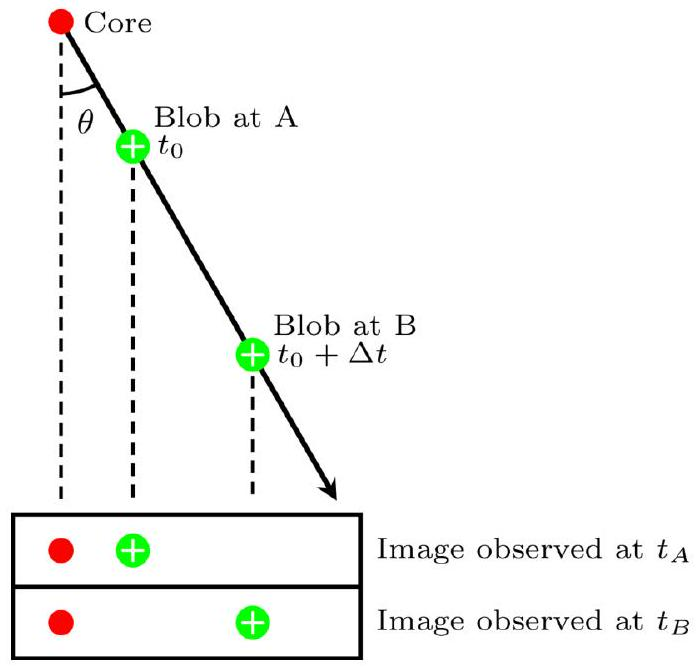
\includegraphics[max width=\textwidth, center]{2025_08_23_e94579452776a99c4850g-04}\\
    (T05.2) The light emitted by the blob at two different times $t_{0}$ (corresponding to position A ) and $t_{0}+\Delta t$ (corresponding to position B ) reaches the observer at $t_{\mathrm{A}}$ and $t_{\mathrm{B}}$, respectively. Thus the observed time difference is $\Delta t_{\text {app }}=t_{\mathrm{B}}-t_{\mathrm{A}}$.\\
    (T05.2a)\\
    Find an expression for the ratio $\frac{\Delta t_{\mathrm{app}}}{\Delta t}$ in terms of $\beta$ and $\theta$.\\
    (T05.2b) Using this ratio, express $\beta_{a p p}$ in terms of $\beta$ and $\theta$.\\
    (T05.3) Motion is called superluminal if the apparent speed exceeds that of light ( $\beta_{\mathrm{app}}>1$ ), and subluminal if it does $\operatorname{not}\left(\beta_{\mathrm{app}}<1\right)$.\\
    (T05.3a) For $\beta_{\mathrm{app}}=1$, plot a smooth curve of $\beta$ as a function of $\theta$ to mark the boundary between subluminal and superluminal motions. Shade the superluminal region in the graph with slanted lines (///).\\
    (T05.3b) Find the lowest true jet speed ( $\beta_{\text {low }}=v_{\text {low }} / c$ ) for the superluminal motion to occur and also its corresponding viewing angle $\theta_{\text {low }}$.\\
    (T05.4) Find an expression for the maximum viewing angle, $\theta_{\max }$, for which a given value of $\beta_{\mathrm{app}}$ will be possible.
    
    The core of a quasar, its central compact object, exhibits variability in its emission due to internal processes occurring within a causally connected region. The size (= radius) of this region is typically taken to be about five times the Schwarzschild radius of the core.\\
    (T05.5) The core of a certain quasar is found to vary on time scales of about 1 h . Obtain an upper limit, $M_{\mathrm{c}, \max }$, on the mass of the central compact object, in units of solar mass.
    

\end{document}